\documentclass[10pt]{beamer}

% Configuration {{{
\usepackage[utf8]{inputenc}
\usepackage[T2A]{fontenc} % T1 for English
\usepackage[english, russian]{babel}

\usepackage{mathtools}
\usepackage{graphicx}
\usepackage{tikz}
\usepackage[multidot]{grffile}
\usepackage[labelsep=period]{caption}
\usepackage{multirow}

\setbeamertemplate{caption}[numbered]
\setbeamertemplate{navigation symbols}{}
\usefonttheme[onlymath]{serif}
\usepackage{DejaVuSansCondensed} % helvet for English
\usetheme{Madrid}

\linespread{1.2}
% }}}

% Title {{{
\title[Проблемы квантовой физики]{%
  Проблема квантовых корреляций, нелокальности, несепарабельности %
  и квантовая информация
}
\author{Керим Гусейнов}
\institute[МГУ]{Московский государственный университет имени М.\,В.~Ломоносова}
\date{28 января 2023 г.}
%}}}

\begin{document}

\frame[plain]{\titlepage}

\begin{frame}[label=interpretations-1]%{{{
  \frametitle{Интерпретации квантовой теории}

  Квантовая теория -- довольно успешный математический аппарат описания 
  определенных систем. Однако не существует единственной онтологической 
  картины квантовой теории.

  \begin{itemize}
    \item Копенгагенская: мы можем быть уверены в реальности лишь 
      конкретных результатов измерений. Некорректно задавать вопрос, 
      например, о существовании электрона.

    \item Дж. Уилер: Вселенная обеспечивает свое существование 
      посредством актов участия наблюдателя. Поведение микрообъекта 
      определяется в момент измерения. Измерение доводит процесс до 
      полноты.

    \item Множественность миров: каждая возможность реализуется 
      в определенном мире. Количество альтернативных миров увеличивается 
      с каждым измерением.
  \end{itemize}
\end{frame}%}}}

\begin{frame}[label=interpretations-2]%{{{
  \frametitle{Интерпретации квантовой теории}

  \begin{itemize}
    \item Квантовологическая: парадоксы квантовой теории не являются 
      проблемами физики, а возникают по вине устаревшей бинарной логики. 
      Логика сознания строится как аппарат, позволяющий справляться 
      с миром. Логика не априорна и должна измениться вместе с картиной 
      мира (аналогично геометрии и СТО/ОТО).

    \item Неореалистская: квантовые эффекты в конечном итоге обусловлены 
      классическими объектами, которые будут видны в более глубокой 
      теории. По-видимому, опровергнуто экспериментами по неравенству 
      Белла.

    \item Само сознание наблюдателя создает реальность, а не 
      измерительный прибор без наблюдателя.

    \item Холистская: Вселенная является единственным целым, а ее части 
      содержат отражение всего мира. Повсюду задан имплицитный порядок.
  \end{itemize}
\end{frame}%}}}

\begin{frame}[label=interpretations-3]%{{{
  \frametitle{Интерпретации квантовой теории}

  \begin{itemize}
    \item Д.И. Блохинцев: центральным понятием является 
      квантовомеханический ансамбль, подобный ансамблю Гиббса. Он 
      образуется повторением ситуации, в которых одинаковая система 
      ставится в одинаковую обстановку. Обстановка диктует состояние 
      квантовой системы, но система объективна.

    \item Интеграл по траекториям Фейнмана говорит о необходимости 
      учитывать все мыслимые траектории системы, соединяющие начальную 
      и конечную точки.

    \item Гейзенберг: копенгагенская интерпретация с замечанием, что 
      квантовые системы реальны и их природа такова, что нужно вернуться 
      к двум модусам бытия: бытие в возможности и бытие действительного.
  \end{itemize}
\end{frame}%}}}

\begin{frame}[label=EPR-paradox]%{{{
  \frametitle{Парадокс Эйнштейна-Подольского-Розена}

  \begin{itemize}
    \item Мысленный эксперимент, демонстрирующий особенности квантовой 
      теории в применении к составным системам (неполнота). Назван 
      парадоксом, поскольку Эйнштейн считал полноту \textit{критерием} 
      физической реальности.

    \item Изначально сформулирован касательно координаты и импульса, но 
      применим к любой паре некоммутирующих наблюдаемых.

    \item Пусть квантовая система состоит из двух частиц, вылетевших 
      с одинаковыми импульсами из одной точки пространства. На пути 
      одной из частиц поставлен прибор, измеряющий координату. На пути 
      другой -- импульс. Авторы утверждают, что при достаточном удалении 
      частиц друг от друга можно (независимо) измерить координату одной 
      и импульс другой, получив таким образом полную информацию, что 
      противоречит принципу неопределенности Гейзенберга.
  \end{itemize}
\end{frame}%}}}

\begin{frame}[label=EPR-experiment]%{{{
  \frametitle{Парадокс ЭПР -- проверка}

  \begin{itemize}
    \item Бом предложил провести аналогичный эксперимент со спинами.
    \item Белл затем вывел неравенство, однозначно демонстрирующее, 
      зависимость (или независимость) измерений. Изначальная форма не 
      так удобна на практике, но позднее были выведены формулы 
      относительно корреляций измерений.
    \item В экспериментах определяется корреляция между поляризацией 
      двух (спутанных) частиц при разных углах поляризаторов $a$ и $b$.
      \\\hfill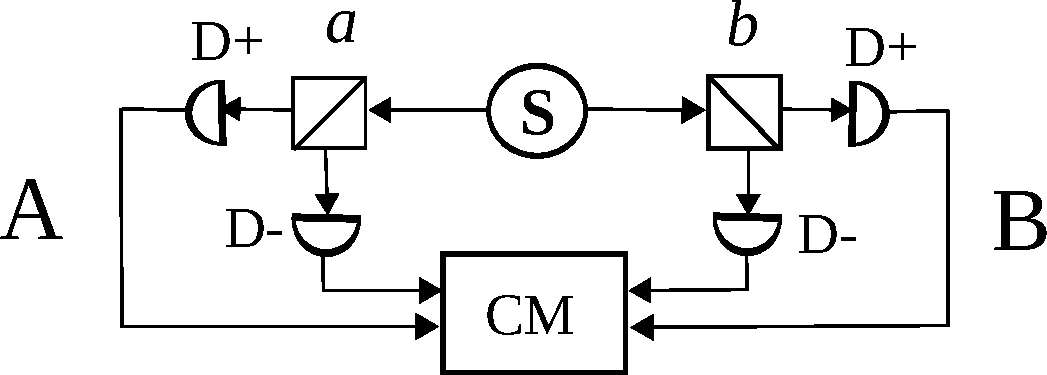
\includegraphics[width=.5\linewidth]{figures/bell-test}
      \hfill\null
    \item За проведенные эксперименты была выдана Нобелевская премия по 
      физике в 2022 году Алену Аспе, Джону Клаузеру и Антону Цайлингеру.
  \end{itemize}
\end{frame}%}}}

\begin{frame}[label=EPR-experiment-opposition]%{{{
  \frametitle{Парадокс ЭПР -- возражения к экспериментам}

  \begin{itemize}
    \item Если детектируются не все частицы, наблюдаемая статистика 
      может не воспроизводить полную. Для полноценного запрета требуется 
      достаточно высокая эффективность регистрации, что представляет 
      проблему в экспериментах с фотонами.

    \item Для полноценного эксперимента измерения должны производиться 
      на пространственноподобных интервалах. То есть приборы должны быть 
      сильно разделены пространственно, а частицы должны долгое время 
      лететь, будучи спутанными. Последнее является проблемой для 
      заряженных частиц.

    \item Регистрируемые частицы могут на самом деле не быть спутанными. 
      Требуется достаточно узкое окно регистрации и низкая частота 
      испускания.
  \end{itemize}
\end{frame}%}}}

\begin{frame}[label=EPR-consequences]%{{{
  \frametitle{Парадокс ЭПР -- значение}

  \begin{itemize}
    \item Нелокальность.
      Нет однозначного согласия на эту тему. Некоторые утверждают, что 
      классическая локальность относится только к непрерывным переменным 
      (координата и импульс) а спин может вести себя экзотично.

      Некоторые утверждают, что нелокальность требует отказаться от 
      СТО/ОТО и теории пространства-времени Эйнштейна вообще.

      Тем не менее нелокальность, даже в полном смысле этого слова, не 
      запрещает физическую реальность квантовой теории (хотя многие 
      интерпретации на нее и не претендуют).

    \item Несепарабельность (целостность).
      Состояние системы невозможно описать измерениями ее частей, даже 
      если включить информацию о всех корреляциях. Считается, что это -- 
      внутреннее свойство теории, обусловленное Гильбертовым 
      пространством.

      Существенный конфликт с понятием объективности, которое требует 
      существования объекта самого по себе.
  \end{itemize}
\end{frame}%}}}

\begin{frame}[label=EPR-Copenhagen-support]%{{{
  \frametitle{Еще одно подтверждение копенгагенской интерпретации}

  \begin{itemize}
    \item Квантовый ластик с отложенным выбором. Вместо регистрации 
      частицы сразу ей придается фаза или что-либо подобное, дающее при 
      дальнейшем измерении возможность узнать, где частица прошла. На 
      деле частица проходит сразу везде.
    \item Подтверждает, что система теряет когерентность из-за наличия 
      информации после измерений.
  \end{itemize}

  \vfill
  \centering
  \def\localheight{.4\textheight}
  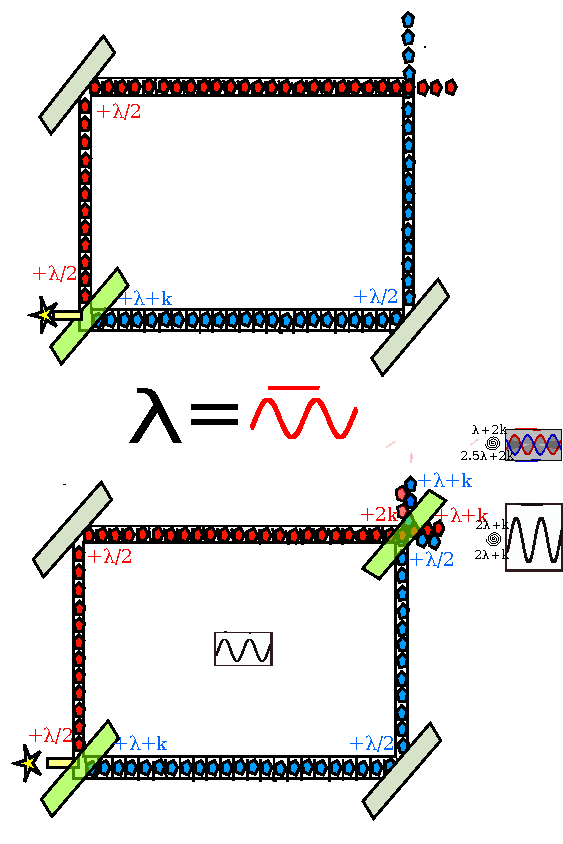
\includegraphics[height=\localheight]{figures/quantum-eraser-classical}
  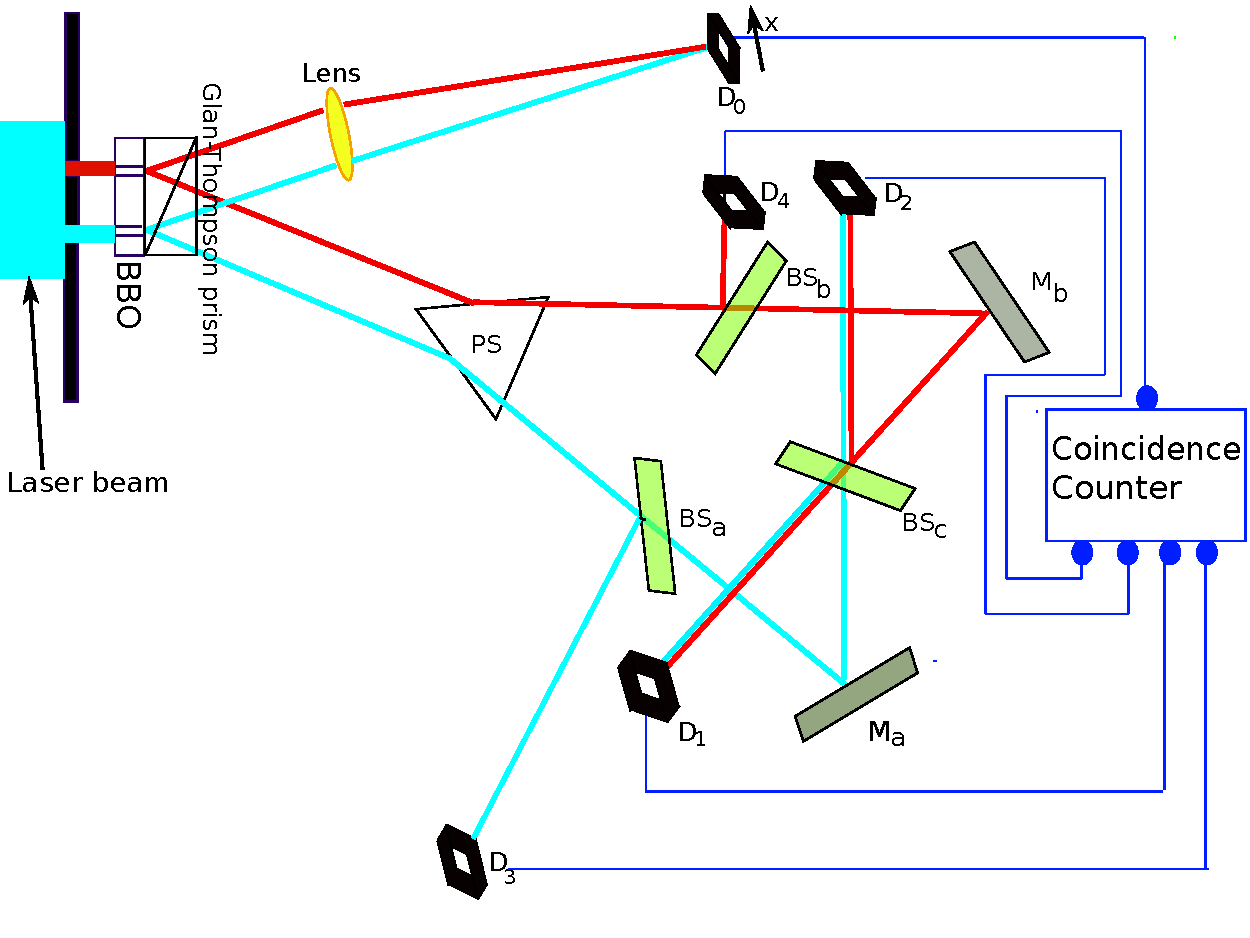
\includegraphics[height=\localheight]{figures/quantum-eraser-nonclassical}
\end{frame}%}}}

\begin{frame}[label=quantum-information]%{{{
  \frametitle{Квантовая информация}

  \begin{itemize}
    \item Возможность сохранить информацию в состоянии квантовой системы 
      аналогично традиционным битам. Принципиальные отличия: 
      суперпозиция и спутанность.
    \item Наиболее развита квантовая криптография, позволяющая исключить 
      подслушивание, поскольку перехват сигнала неизбежно приводит 
      к искажению, которое было бы заметно отправителю при проверке.
    \item Квантовая телепортация (информации) не позволяет передавать 
      данные быстрее скорости света, поскольку требует вспомогательных 
      классических данных.

      Квантовая телепортация позволяет реконструировать зашифрованное 
      состояние частицы на основе конкретного измерения, которое должно 
      быть согласовано у отправителя и получателя.
  \end{itemize}
\end{frame}%}}}

\begin{frame}[label=conclusions]%{{{
  \frametitle{Выводы}

  \begin{itemize}
    \item Квантовая физика предоставила серьезный вызов философии.
    \item Многочисленные интерпретации квантовой теории до сих пор 
      соревнуются между собой.
    \item В большинстве интерпретаций можно выделить конструктивизм.
    \item Радикальные направления (конструктивизм, холизм) содержат 
      противоречия и приняты наиболее узко.
    \item Копенгагенская интерпретация наиболее популярна, хоть на ней 
      никто и не хочет останавливаться.
    \item Проблемы нелокальности и несепарабельности требуют глубокого 
      анализа, как философского, так и физического.
  \end{itemize}
\end{frame}%}}}

\end{document}

Фразы:

- Поппер пишет, что действие на расстоянии потребовало бы переосмысления 
  времени, а это в свою очередь ставит под вопрос теорию эволюции 
  и подобные дела. Я думаю, что нельзя говорить о теории эволюции 
  и биологии на этом уровне, ставить их в аргумент и в защиту какой-либо 
  истины, поскольку физика гораздо более продвинута и гораздо глубже 
  рассматривает. Это похоже на оппозицию гелиоцентризму со стороны 
  повседневного опыта восходов и закатов.

- Нарушение нелокальности по Бэллу не ведет к экспериментально
  обнаруживаемому действию. Не было бы телеграфа Бэлла.
- Может не быть соответствия классич. одновременности и локальности
  по Бэллу.
